\documentclass[conference]{IEEEtran}
\IEEEoverridecommandlockouts
\usepackage{cite}
\usepackage{balance}
\usepackage{amsmath,amssymb,amsfonts}
\usepackage{graphicx}
\usepackage{textcomp}
\usepackage{xcolor}
\usepackage{booktabs}
\usepackage{array}
\usepackage{algorithm}
\usepackage{algorithmic}
\usepackage{tikz}
\usetikzlibrary{positioning,arrows.meta,calc}
\usepackage[hidelinks]{hyperref}
\input{nums.tex}

\begin{document}

\title{Checking Every Proposal: A Fail-Closed Flood\\
Decision-Support Chain from Forecast to Dispatch}

%<AUTHORS>
\author{
\IEEEauthorblockN{Nandhakumar T}
\IEEEauthorblockA{\textit{Department of Information Technology}\\
\textit{Sona College of Technology}\\
Salem, Tamil Nadu, India\\
nandhakumartm93@gmail.com}
\and
\IEEEauthorblockN{Balakarthikeyan B S}
\IEEEauthorblockA{\textit{Department of Artificial Intelligence and Data Science}\\
\textit{Sona College of Technology}\\
Salem, Tamil Nadu, India\\
balasan2626@gmail.com}
\and
\IEEEauthorblockN{Gowthaman J}
\IEEEauthorblockA{\textit{Department of Artificial Intelligence and Data Science}\\
\textit{Sona College of Technology}\\
Salem, Tamil Nadu, India\\
gowthamanjanadhran@gmail.com}
\and
\IEEEauthorblockN{Abhishek S}
\IEEEauthorblockA{\textit{Department of Artificial Intelligence and Data Science}\\
\textit{Sona College of Technology}\\
Salem, Tamil Nadu, India\\
abisheksengodan18@gmail.com}
}
%</AUTHORS>

\maketitle

\begin{abstract}
Flood decision-support software now combines components whose output can be wrong without warning: a learned forecaster, sampling optimizers such as the Quantum Approximate Optimization Algorithm (QAOA), and large language models (LLMs) that narrate the situation. We describe a prototype in which each of these components may only propose, and a deterministic check at its boundary decides what reaches the emergency officer. We evaluate every check on measured data. A gradient-boosted forecaster scored on CAMELS-IND gauges unseen in space and time reached a balanced accuracy of \FcXgbBA{} for three-day flood exceedance, against \FcLstmBA{} for the dataset's LSTM simulation; a random row split would have reported \FcLeakRandBA. For shelter re-planning, a constraint-preserving mixer raised QAOA's probability of the optimal plan from at most \QaSeedXMax{} to \QaSeedXYMean, and angles fixed in advance served new disruptions without retraining. Even so, the most frequent sample of an unchecked loop was invalid in \RaTwinRawQ\% of re-planning events for QAOA and \RaTwinRawSA\% for simulated annealing. An exact verifier backed by a mixed-integer certificate dispatched no invalid plan, and all \RaCityTimeout{} solver time-outs turned out to hide valid plans. In the agent layer, a composed check found that dispatch bypassed the verified policy in \AgEtoEViolBefore{} of \AgEtoECases{} cases, and \AgLiveUnsupPct\% of \AgLiveN{} live LLM replies stated a number absent from the state; a slot-typed guard caught \AgLiveTypRec\% of them. All quantum results are classical simulations and imply no quantum advantage.
\end{abstract}

\begin{IEEEkeywords}
flood forecasting, runtime assurance, QAOA, large language models, fail-safe design, evacuation planning
\end{IEEEkeywords}

\section{Introduction}
During a flood, an emergency operations centre turns a forecast into a decision, the decision into a shelter plan and the plan into radio messages. Each step is now offered to a new kind of component: data-driven forecasters trained on many catchments \cite{Kratzert2019a,Nearing2024}, quantum and quantum-inspired optimizers for assignment problems \cite{Lucas2014,Abbas2024,Cadelina2024}, and LLMs that plan, call tools and speak \cite{Yao2023}. They fail in different ways. A forecaster's reported skill depends on how its test data were split \cite{Kapoor2023,Roberts2017}. A sampler returns candidates, not proven answers, and the penalty encodings it needs for capacity limits are exact only in special cases \cite{Glover2019}. An LLM can state numbers its input does not contain \cite{Ji2023}.

Safety engineering has a standard answer for unreliable parts: keep them, but put a simple checked element between them and the action \cite{Sha2001,Desai2019}, as shields do for learned policies \cite{Alshiekh2018}, and choose the level of automation per function \cite{Parasuraman2000}. For a whole flood system three questions remain open. Does each check hold on the path to action as it is actually built? What does each check cost in false alarms and lost quality? And what should the system do when a check cannot decide?

We study these questions on an open flood decision-support prototype with a digital twin of the Delhi Yamuna corridor, OpenStreetMap road networks of six Indian cities and a forecasting benchmark on CAMELS-IND \cite{Mangukiya2025}. Our contributions are:
\begin{enumerate}
\item A fail-closed chain in which the forecaster, the re-planner and the narrator can only propose, and a deterministic check at each boundary decides what reaches the officer (Fig.~\ref{fig:chain}, Table~\ref{tab:layers}).
\item A forecast evaluation on gauges held out in space and time, with the effect of the evaluation protocol measured.
\item Shelter re-planning with QAOA under a constraint-preserving mixer and transferable angles, run inside a runtime-assurance loop with exact verification and a certificate for escalation.
\item Measurements on the deployed agent code: a composed check from policy to dispatch, and the grounding of live LLM replies under three guards.
\end{enumerate}

\section{Related Work}
\textit{Forecasting.} Long short-term memory (LSTM) networks trained on large-sample data simulate streamflow well, even in ungauged basins \cite{Kratzert2019a,Nearing2024}. Random row splits let days of one flood fall on both sides of the split, which inflates scores \cite{Kapoor2023,Roberts2017}; we score on gauges and years that played no part in training.

\textit{Quantum optimization.} QAOA alternates a cost and a mixing unitary \cite{Farhi2014}; constraint-preserving mixers keep the state among feasible plans \cite{Hadfield2019,WangZ2020}, and rescaled instances can share one set of angles \cite{Shaydulin2023}. These studies use equality constraints or unconstrained MaxCut, whereas shelter capacity is an inequality. Quantum annealing has been applied to disaster resource allocation with a penalty encoding and no check of the returned samples \cite{Cadelina2024}.

\textit{Runtime assurance and LLM guards.} The Simplex architecture lets a verified controller replace a complex one \cite{Sha2001}, and SOTER brings this to robotics software \cite{Desai2019}. For LLMs, programmable rails \cite{Rebedea2023} and runtime enforcement for agents \cite{WangH2026} restrict what a model may do, and a second LLM can act as a judge \cite{Zheng2023}. Safety, however, is a property of the whole control structure \cite{Leveson2011}. To our knowledge no flood system has been evaluated with checks on its forecaster, its optimizer and its narrator together, on the code that runs.

\section{System}\label{sec:sys}
The prototype runs one pipeline per tick, either on live weather and river data or on a digital twin of the corridor. Eleven agents share one state object and write every event to a log, so the officer sees what each agent did and why. Fig.~\ref{fig:chain} shows the chain. The rule is the same at every layer: a component that can be wrong produces a proposal, and a deterministic check decides whether it passes, is replaced by a safe default or goes to a human. Checks can hold, downgrade or reject; none can start an action. Table~\ref{tab:layers} summarises each layer and its main measured result, which Sections~\ref{sec:fc}--\ref{sec:ag} report in turn.

\begin{figure}[t]
\centering
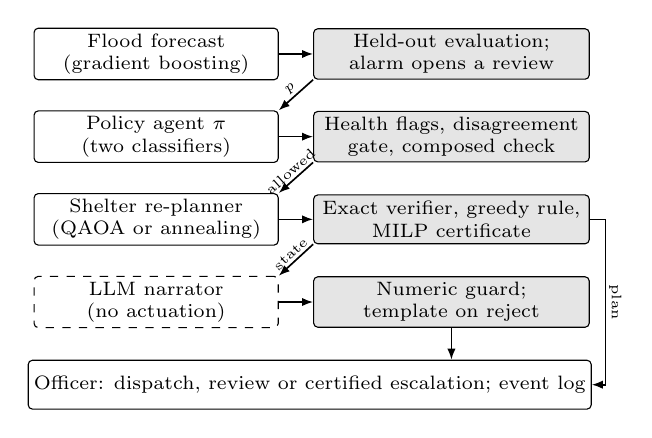
\begin{tikzpicture}[font=\scriptsize,
  box/.style={draw, rounded corners=1.5pt, align=center, minimum width=3.1cm, minimum height=0.62cm, inner sep=2pt},
  chk/.style={box, fill=gray!20, minimum width=3.5cm},
  arr/.style={-{Latex[length=1.4mm]}, semithick}, lab/.style={font=\tiny, inner sep=1pt}]
\node[box] (fc) at (0,0) {Flood forecast\\(gradient boosting)};
\node[chk] (c1) at (3.75,0) {Held-out evaluation;\\alarm opens a review};
\node[box] (pol) at (0,-1.05) {Policy agent $\pi$\\(two classifiers)};
\node[chk] (c2) at (3.75,-1.05) {Health flags, disagreement\\gate, composed check};
\node[box] (opt) at (0,-2.1) {Shelter re-planner\\(QAOA or annealing)};
\node[chk] (c3) at (3.75,-2.1) {Exact verifier, greedy rule,\\MILP certificate};
\node[box, dashed] (llm) at (0,-3.15) {LLM narrator\\(no actuation)};
\node[chk] (c4) at (3.75,-3.15) {Numeric guard;\\template on reject};
\node[box, minimum width=7.0cm] (off) at (1.95,-4.2) {Officer: dispatch, review or certified escalation; event log};
\draw[arr] (fc) -- (c1);
\draw[arr] (pol) -- (c2);
\draw[arr] (opt) -- (c3);
\draw[arr] (llm) -- (c4);
\draw[arr] (c1.south west) -- node[lab, above, sloped]{$p$} (pol.north east);
\draw[arr] (c2.south west) -- node[lab, above, sloped]{allowed} (opt.north east);
\draw[arr] (c3.south west) -- node[lab, above, sloped]{state} (llm.north east);
\draw[arr] (c4) -- (c4 |- off.north);
\draw[arr] (c3.east) -- ++(0.2,0) |- node[lab, pos=0.25, above, sloped]{plan} (off.east);
\end{tikzpicture}
\caption{The fail-closed chain. Left: components that can be wrong and only propose. Shaded: the deterministic check at each boundary, which can hold, downgrade or reject but never act. The LLM (dashed) narrates the logged state and has no actuation rights.}
\label{fig:chain}
\end{figure}

\begin{table}[t]
\caption{Layers of the chain, their checks and the main measured result}
\label{tab:layers}
\centering
\footnotesize
\setlength{\tabcolsep}{2.5pt}
\begin{tabular}{>{\raggedright\arraybackslash}p{1.25cm}>{\raggedright\arraybackslash}p{1.5cm}>{\raggedright\arraybackslash}p{2.35cm}>{\raggedright\arraybackslash}p{2.9cm}}
\toprule
Layer & Proposes & Check & Result\\
\midrule
Forecast (\S\ref{sec:fc}) & flood within 3 days & unseen gauges and years; review on alarm & BA \FcXgbBA, precision \FcXgbPrec\\
Re-planner (\S\ref{sec:qa}, \S\ref{sec:ra}) & shelter plan (samples) & exact verifier, greedy rule, MILP & 0 invalid plans dispatched; \RaCitySettled/\RaCityN{} cases certified\\
Policy (\S\ref{sec:ag}) & dispatch & health flags, gate, composed check & bypasses \AgEtoEViolBefore{} $\rightarrow$ \AgEtoEViolAfter\\
Narrator (\S\ref{sec:ag}) & radio text & typed numeric guard & recall \AgLiveTypRec\%, false rejection \AgLiveTypFpr\%\\
\bottomrule
\end{tabular}
\end{table}

\section{Forecast Layer}\label{sec:fc}
\textit{Task and split.} For gauge $g$ on day $t$ the target is
\begin{equation}
y_{g,t}=\mathbb{1}\Big[\max_{h\in\{1,2,3\}} Q_{g,t+h}\ \ge\ q^{95}_g\Big],
\label{eq:target}
\end{equation}
where $Q$ is observed streamflow and $q^{95}_g$ the 95th percentile of the gauge's flow in the training years only. The \FcNFeat{} inputs (streamflow, rainfall, weather, soil moisture, season and catchment attributes) are all known at the end of day $t$. We train on \FcNTrainGauges{} gauges for 1980--2008, select the model and its decision threshold on 2009--2014, and test once on \FcNTestGauges{} unseen gauges in 2015--2020, labelled by (\ref{eq:target}) (\FcNTestRows{} gauge-days, \FcPosRate\% flood windows). A depth-6 XGBoost model \cite{Chen2016} won the validation comparison.

\textit{Results.} Table~\ref{tab:fc} compares it with persistence, the gauge's own climatology and the CAMELS-IND regional LSTM simulation, which is driven by the observed future rain and so has an advantage no forecaster has. The model led on balanced accuracy (BA) and on PR-AUC (Fig.~\ref{fig:pr}). Scored on random rows instead, the same configuration reached a BA of \FcLeakRandBA{} and a PR-AUC of \FcLeakRandPR, against \FcLeakSpTiBA{} and \FcLeakSpTiPR{} on the held-out split (both from the 500,000-row refit used for the protocol comparison): the protocol alone moved PR-AUC by \FcLeakGapPR{} points. Streamflow inputs carried \FcImpFlow\% of the model's gain, and recall fell from \FcLeadOne\% one day ahead to \FcLeadThree\% three days ahead. Skill rose with catchment area (Spearman $\rho=\FcRhoArea$, $p=\FcPArea$), and \FcFpMonsoonPct\% of false alarms came in the monsoon.

\begin{table}[t]
\caption{Three-day flood exceedance on \FcNTestGauges{} unseen gauges, 2015--2020}
\label{tab:fc}
\centering
\footnotesize
\setlength{\tabcolsep}{3.5pt}
\begin{tabular}{lcccc}
\toprule
Model & BA (95\% CI) & PR-AUC & Recall & Precision\\
\midrule
XGBoost (selected) & \FcXgbBA{} (\FcXgbBALo--\FcXgbBAHi) & \FcXgbPR & \FcXgbRec & \FcXgbPrec\\
XGBoost, no flow & \FcNoFlowBA{} (\FcNoFlowBALo--\FcNoFlowBAHi) & \FcNoFlowPR & \FcNoFlowRec & \FcNoFlowPrec\\
LSTM simulation & \FcLstmBA{} (\FcLstmBALo--\FcLstmBAHi) & \FcLstmPR & \FcLstmRec & \FcLstmPrec\\
Climatology & \FcClimBA{} (\FcClimBALo--\FcClimBAHi) & \FcClimPR & \FcClimRec & \FcClimPrec\\
Persistence & \FcPersBA{} (\FcPersBALo--\FcPersBAHi) & \FcPersPR & \FcPersRec & \FcPersPrec\\
\bottomrule
\multicolumn{5}{l}{\scriptsize CI: gauge-cluster bootstrap. LSTM simulation uses observed future rain.}\\
\end{tabular}
\end{table}

\begin{figure}[t]
\centering
\includegraphics[width=\columnwidth]{fig_fc_pr.pdf}
\caption{Precision--recall curves on the unseen test gauges. The square is persistence; the dotted line is the flood rate.}
\label{fig:pr}
\end{figure}

\textit{Check.} A precision of \FcXgbPrec{} means that most alarms are false, so in the chain an alarm opens a review and never an order. The model without streamflow inputs is the fallback for a lost gauge feed: its BA was lower, \FcNoFlowBA, but it warned of \FcEvNoFlowWarn\% of the \FcEvN{} flood onsets in advance, against \FcEvXgbWarn\% for the full model, because onsets depend on rain more than on the current river state. In the chain, the data-health flag that the policy agent reads (Section~\ref{sec:ag}) would switch the forecast to this fallback; this switch is designed but not yet built. The raw probabilities were \FcCalWord{} (expected calibration error, ECE, \FcEceRaw): in the highest well-populated bin the forecast averaged \FcRelHiConf{} while floods followed in \FcRelHiFreq{} of cases. Isotonic recalibration fitted on validation data lowered the ECE to \FcEceIso{} (Fig.~\ref{fig:rel}), so the number shown to an officer can be read as a frequency.

\begin{figure}[t]
\centering
\includegraphics[width=\columnwidth]{fig_fc_rel.pdf}
\caption{Reliability of the forecast probabilities on the unseen test gauges, before and after isotonic recalibration fitted on validation data (bins with at least 50 gauge-days).}
\label{fig:rel}
\end{figure}

\section{Shelter Re-Planning with QAOA}\label{sec:qa}
\textit{Formulation.} Groups $g$ of size $n_g$ are assigned to shelters $s$ with $R_s$ seats left. With travel cost $c_{gs}$ on the best open path (flood- and congestion-weighted) and a set $\mathcal F$ of forbidden pairs (no open path, failed shelter, group larger than the seats left), a plan $\mathbf x\in\{0,1\}^{G\times S}$ is valid when
\begin{multline}
V(\mathbf x)=\Big[\textstyle\sum_s x_{gs}=1\ \forall g\Big]\wedge\Big[x_{gs}=0\ \forall (g,s)\in\mathcal F\Big]\\
\wedge\Big[\textstyle\sum_g n_g x_{gs}\le R_s\ \forall s\Big].
\label{eq:valid}
\end{multline}
Capacity is an inequality that normally needs slack qubits. We encode it pairwise instead: with $\mathcal O$ the pairs of groups that together exceed $R_s$ and shifted costs $c'_{gs}=c_{gs}-\min_{s'}c_{gs'}$,
\begin{multline}
E(\mathbf{x})=\sum_{g,s}c'_{gs}x_{gs}+P\Big[\sum_g\Big(1-\sum_s x_{gs}\Big)^2\\
+\sum_{(g,s)\in\mathcal{F}}x_{gs}\\
+\sum_{(g,h,s)\in\mathcal{O}}x_{gs}x_{hs}\Big].
\label{eq:qubo}
\end{multline}
After scaling every instance to the energy range $[0,1]$, all instances share one scale. The pairwise term cannot see an overload by three or more groups whose pairs all fit, so a minimum of (\ref{eq:qubo}) need not satisfy (\ref{eq:valid}); Section~\ref{sec:ra} measures how often this happens.

\textit{Mixers and transfer.} We simulate QAOA \cite{Farhi2014} exactly on 12-qubit twin instances (four groups, three shelters) after a road closure and a shelter surge. The transverse-field (X) mixer explores all bitstrings; a ring-XY mixer \cite{Hadfield2019,WangZ2020} swaps amplitude inside each group, so every state stays a one-hot plan; a Grover mixer \cite{Bartschi2020} mixes all one-hot plans in one step but needs far deeper circuits. For transfer, we fix at each depth the trained angle set that works best on average over \QaNPaired{} development instances, in the spirit of \cite{Shaydulin2023}, and apply it unchanged to new instances.

\textit{Results.} Over \QaNPaired{} instances and \QaNSeeds{} optimizer seeds, the XY mixer placed \QaSeedXYMean{}~$\pm$~\QaSeedXYSd{} of its probability on the optimal plan at depth 4, against at most \QaSeedXMax{} for the X mixer, and beat it on at least \QaStXYvXWinsMin{} of \QaNPaired{} instances at every depth (Holm-adjusted $p\le\QaStXYvXMaxP$). The Grover mixer was not significantly different from XY ($p\ge\QaStXYvGMMinP$). Fig.~\ref{fig:popt} shows the trend with depth and Table~\ref{tab:qa} the transfer. On \QaHoN{} held-out twin instances the fixed angles beat per-instance training, at no per-instance cost. On \QaCityN{} instances built on the road graphs of \QaCityNCities{} cities they matched it ($p=\QaCityP$) and found the optimum within \QaShots{} shots far more often. In a scaling run at depth 2 the XY mixer stayed above uniform sampling of one-hot plans up to \QaScaleMaxQ{} qubits, while the X mixer fell below it from 12 qubits on.

\textit{Classical baselines.} Exhaustive search over the 81 one-hot plans took \QaExactMs~ms per instance. A greedy rule found a feasible plan in \QaGreedyFeas\% of instances and the optimum in \QaGreedyOpt\%, and simulated annealing with 20 restarts reached the optimum in \QaSATunedOpt\% in \QaSATunedMs~ms. QAOA is therefore not the fastest or the most reliable solver at this size. The results show which formulation and training choices a hardware study should use, and Section~\ref{sec:ra} shows why even a good sampler cannot be trusted alone.

\begin{figure}[t]
\centering
\includegraphics[width=\columnwidth]{fig_qa_popt.pdf}
\caption{Probability of the optimal plan (left) and of any feasible plan (right) against QAOA depth. The dotted line is uniform sampling of one-hot plans.}
\label{fig:popt}
\end{figure}

\begin{table}[t]
\caption{Angle transfer at depth 4 (XY mixer, 12 qubits)}
\label{tab:qa}
\centering
\footnotesize
\setlength{\tabcolsep}{4pt}
\begin{tabular}{lcc}
\toprule
Measure & Trained per instance & Fixed angles\\
\midrule
Held-out twin, $P_{\mathrm{opt}}$ & \QaHoTrainedFour & \QaHoFixedFour\\
Held-out, optimum in \QaShots{} shots (\%) & \QaHoSuccTrained & \QaHoSuccFixed\\
Held-out, circuit evaluations & \QaHoCumFour & 0\\
Six cities, $P_{\mathrm{opt}}$ & \QaCityTrained & \QaCityFixed\\
Cities, optimum in \QaShots{} shots (\%) & \QaCitySuccTrained & \QaCitySuccFixed\\
\bottomrule
\end{tabular}
\end{table}

\section{Runtime Assurance for the Re-Planner}\label{sec:ra}
A good sampler is still a sampler. Algorithm~\ref{alg:loop} puts it inside a runtime-assurance loop \cite{Sha2001,Desai2019}. Every sample is checked with (\ref{eq:valid}) against the state at dispatch time. If none passes, a greedy rule (largest group first to its cheapest shelter with seats left) is tried. Only then does the loop ask a mixed-integer program (MILP), solved with HiGHS \cite{Huangfu2018}, to minimise $\sum c_{gs}x_{gs}$ subject to (\ref{eq:valid}). An infeasible MILP certifies that no valid plan exists, so the escalation to a human is justified; a feasible one supplies the plan. A solver time-out proves nothing, so that case is escalated but marked uncertified. The natural baseline is the uncertified loop, which escalates whenever the sampler and the greedy rule fail.

\begin{algorithm}[t]
\caption{Runtime-assurance re-planning at one event}
\label{alg:loop}
\begin{algorithmic}[1]
\small
\STATE draw shots in batches until a sample passes $V$ or the budget is used
\STATE $\mathbf x\leftarrow$ cheapest sample with $V(\mathbf x)$; \textbf{if} none, $\mathbf x\leftarrow$ greedy
\IF{$V(\mathbf x)$}
\STATE dispatch $\mathbf x$
\ELSE
\STATE solve the MILP with a time limit; \textbf{if} feasible, dispatch its plan
\STATE \textbf{if} infeasible, escalate with the certificate; \textbf{if} timed out, escalate as uncertified
\ENDIF
\end{algorithmic}
\end{algorithm}

\textit{Setup.} On the twin we replay \RaTwinSeeds{} seeded episodes of closures, a shelter surge and two shelter failures (\RaTwinEvents{} events, \RaTwinInfeasible{} without any valid plan), each sampled ten times by depth-3 XY QAOA and by simulated annealing \cite{Kirkpatrick1983} on the same QUBO. At city scale we built \RaCityN{} instances on the road graphs of the six cities with 8, 16 or 32 groups and ten shelters (\RaCityMinVars--\RaCityMaxVars{} variables), where enumeration is impossible and the MILP is the only exact reference.

\begin{table}[t]
\caption{Re-planning with and without the checks}
\label{tab:ra}
\centering
\footnotesize
\setlength{\tabcolsep}{3pt}
\begin{tabular}{lc}
\toprule
Measure & Value\\
\midrule
\multicolumn{2}{l}{\textit{Twin: \RaTwinEvents{} events $\times$ 10 draws, 12 variables}}\\
Unchecked top sample invalid, QAOA (\%) & \RaTwinRawQ{} (\RaTwinRawQLo--\RaTwinRawQHi)\\
Unchecked top sample invalid, annealing (\%) & \RaTwinRawSA{} (\RaTwinRawSALo--\RaTwinRawSAHi)\\
Invalid samples the penalty could not see, QAOA (\%) & \RaViolBlindQ\\
Invalid plans dispatched by the loop & 0\\
\midrule
\multicolumn{2}{l}{\textit{Cities: \RaCityN{} instances, \RaCityMinVars--\RaCityMaxVars{} variables}}\\
Annealing finds a valid plan, 8 / 32 groups (\%) & \RaCitySAFoundEight{} / \RaCitySAFoundThirtyTwo\\
Solvable cases escalated, uncertified loop (\%) & \RaCityFalseEsc{} (\RaCityFalseLo--\RaCityFalseHi)\\
Settled by MILP within \RaCityLimitS~s & \RaCitySettled{} of \RaCityN\\
Time-outs with a valid plan (\RaLongLimitS~s re-run) & \RaTimeoutFeasible{} of \RaCityTimeout\\
\bottomrule
\multicolumn{2}{l}{\scriptsize Brackets: 95\% intervals from resampling events or instances.}\\
\end{tabular}
\end{table}

\textit{Results.} Table~\ref{tab:ra} gives the outcome. On the twin, dispatching the most frequent sample unchecked would have sent an invalid plan in \RaTwinRawQ\% of event draws for QAOA and \RaTwinRawSA\% for annealing (\RaTwinRawFeasQ\% and \RaTwinRawFeasSA\% on solvable events only). Almost all of these samples overfilled a shelter in exactly the way the pairwise penalty cannot see, so the error lies in the encoding, not in the search. At city scale the search failed instead: the annealer's rate of valid plans on solvable instances fell from \RaCitySAFoundEight\% at 8 groups to \RaCitySAFoundThirtyTwo\% at 32 (Fig.~\ref{fig:city}), and the uncertified loop would have called a human for \RaCityFalseEsc\% of cases that had a plan. The MILP settled \RaCitySettled{} instances, the slowest in \RaMilpMaxS~s. The other \RaCityTimeout{} timed out; re-run with a \RaLongLimitS~s limit, all had valid plans, found within \RaTimeoutMaxS~s. An adaptive shot budget cut the twin's shots per event from 64 to \RaAdaptShots{} with identical escalation decisions, but optimal QAOA plans fell from \RaFixedOptQ\% to \RaAdaptOptQ\% of events.

\textit{Differences between cities.} \RaByCityText{} The MILP's median solve time grew from \RaMilpMedEight~s at 8 groups to \RaMilpMedThirtyTwo~s at 32, so at the sizes tested the certificate costs seconds at most.

\begin{figure}[t]
\centering
\includegraphics[width=\columnwidth]{fig_ra_city.pdf}
\caption{City scale: share of calls in which the sampler produced a valid plan, and share of solvable cases an uncertified loop would escalate, against the number of groups.}
\label{fig:city}
\end{figure}

\section{Agents and LLM Narration}\label{sec:ag}
\textit{Policy and gate.} The Flood Risk agent maps a flood probability $p$ and three health flags (data available, model returned a value, database connected) to one of five actions. With a monitor threshold $\tau_m=0.50$ and an automation threshold $\tau_a=0.60$, the policy $\pi$ returns \textsc{monitor} below $\tau_m$, \textsc{auto} only when $p\ge\tau_a$, all flags are healthy and automation is enabled, \textsc{review} otherwise, and \textsc{override} or \textsc{unavailable} when an operator overrides or no probability exists. A Random Forest \cite{Breiman2001} and an XGBoost classifier score the same features; dispatch is held when they differ by at least 0.15 or fall on opposite sides of $\tau_a$ (the straddle rule).

\textit{Composed check.} An exhaustive test of $\pi$ over \AgPolCases{} cases ($1{,}002$ probability values including an undefined one, eight health combinations and two override states) found \AgPolViol{} violations. The path from policy to dispatch was a different matter. Enumerating \AgEtoECases{} cases through the dispatch code ($1{,}001$ defined probabilities, eight health combinations, two override states and the two states of the hold) showed that teams were sent in \AgEtoEViolBefore{} cases in which the verified policy asked for review, all of them high-probability states with a failed health check: dispatch tested the probability band and the gate but never read the action returned by $\pi$. After the fix (dispatch requires \textsc{auto} or \textsc{override}) the same check found \AgEtoEViolAfter. On \AgCalTest{} held-out rows of the classifiers' data, cases held by the gate were wrong \AgGateDepErrRatio{} times as often as released ones; the gate caught \AgGtDepRecall\% of the policy model's errors. The straddle rule alone held fewer cases (\AgGateStHold\% against \AgGateDepHold\%) with a higher error rate among them, but it caught only \AgGtStRecall\% of the errors, so it is not a better gate.

\textit{Numeric guard.} The LLM receives the logged state and must use only its numbers; it has no actuation rights. The deployed guard accepts a reply only if every number in it matches some number of the prompt up to the rounding written, and replaces a rejected reply by a template filled from the same state. Because it is untyped, a rainfall value quoted as a river level passes. A slot-typed guard first binds each number to a quantity (percent to a probability, mm to rainfall, m to a level, clock times to the current time) and rejects any number it cannot bind.

\textit{Live replies.} We collected \AgLiveN{} replies from gpt-oss-20b and gpt-oss-120b on \AgLiveStates{} seeded flood states. \AgLiveUnsup{} of them (\AgLiveUnsupPct\%) stated at least one unsupported number, and \AgLiveEta{} of those were invented arrival times, although the prompt contains none. A revised typed guard was frozen, with its hash recorded, before replies from a third model family, ALLaM-2 (7B), were collected. Table~\ref{tab:guard} gives the results. The typed guard caught more errors than the deployed one but rejected more correct replies. An LLM judge \cite{Zheng2023} caught nearly all errors; it rejected \AgLiveJJudFpr\% of correct replies when its \AgJudFailN{} failed calls count as rejections and \AgJudAnsFpr\% without them, and it needs a model call per message. On the held-out family the revised guard was not significantly better than the deployed one (McNemar $p=\AgMcVtwoRecP$), and its false rejections rose from \AgDevVtwoFpr\% to \AgHoVtwoFpr\%. No numeric guard sees qualitative over-claims such as ``flood confirmed, made in \AgOcDevPct\% of replies. The kind of error also changed with the model (Fig.~\ref{fig:err}): invented arrival times appeared in \AgErrOssEtaMin--\AgErrOssEtaMax\% of the gpt-oss replies but in only \AgErrAllamEta\% of the ALLaM-2 replies, which instead invented quantities in \AgErrAllamQty\% and misquoted a probability in \AgErrAllamProb\%. A guard tuned to the errors of one model family will therefore miss some errors of the next one, and a typed check of every quantity is safer than a list of known mistakes.

\begin{figure}[t]
\centering
\includegraphics[width=\columnwidth]{fig_ag_errtypes.pdf}
\caption{Kinds of unsupported numbers in live replies, as a share of each model's replies (reference labels). A reply can contain more than one kind.}
\label{fig:err}
\end{figure}

\textit{Classifier calibration.} The disagreement gate held many cases because the two classifiers were calibrated differently: on the held-out rows the XGBoost policy model had an ECE of \AgEceXgb, against \AgEceRf{} for the Random Forest. Isotonic calibration on the training split lowered these to \AgEceCalXgb{} and \AgEceCalRf{} and the hold rate of the deployed rule to \AgGateCalHold\%. The forecast layer and the gate thus need the same repair before their probabilities are compared with a fixed threshold.

\begin{table}[t]
\caption{Guards on live LLM replies: recall on replies with an unsupported number and false rejection (FR) of correct replies, in \%}
\label{tab:guard}
\centering
\footnotesize
\setlength{\tabcolsep}{3.5pt}
\begin{tabular}{lcccc}
\toprule
 & \multicolumn{2}{c}{gpt-oss (\AgLiveN)} & \multicolumn{2}{c}{ALLaM-2, held out (\AgHoN)}\\
Guard & Recall & FR & Recall & FR\\
\midrule
Deployed (untyped) & \AgDevDepRec & \AgDevDepFpr & \AgHoDepRec & \AgHoDepFpr\\
Slot-typed & \AgDevTypRec & \AgDevTypFpr & \AgHoTypRec & \AgHoTypFpr\\
Slot-typed v2 (frozen) & \AgDevVtwoRec & \AgDevVtwoFpr & \AgHoVtwoRec & \AgHoVtwoFpr\\
LLM judge & \AgLiveJJudRec & \AgLiveJJudFpr & -- & --\\
\bottomrule
\multicolumn{5}{l}{\scriptsize v2 was written after reading the gpt-oss replies; -- = not run.}\\
\end{tabular}
\end{table}

\section{Discussion}
Four lessons recur across the layers.

\textit{Check the composed path, not only the component.} The verified policy had no violations, yet the dispatch code bypassed it in \AgEtoEViolBefore{} cases. The forecaster's score depended on the split in the same way: random rows added \FcLeakGapPR{} points of PR-AUC that a new river would never deliver. In both cases the component was correct and the path around it was not.

\textit{Check proposals against typed state.} The two generative components failed for parallel reasons. The pairwise penalty could not see a three-group overload, and the untyped guard could not see a correct number placed in the wrong slot. Both checks compared the output with the right data at the wrong granularity. An exact verifier of (\ref{eq:valid}) and a typed guard close these gaps, because each checks every constraint or quantity by name.

\textit{A check that cannot decide must say so.} A MILP time-out is not a proof of infeasibility, and all \RaCityTimeout{} of ours hid valid plans. The loop therefore escalates such cases marked as uncertified, and the forecaster's alarms go to review because its precision is \FcXgbPrec.

\textit{Every check has a price.} The typed guard rejected \AgLiveTypFpr\% of correct replies against \AgLiveDepFpr\% for the deployed one; the adaptive shot budget lost optimal plans; the no-flow fallback lost BA. We report these costs so that an operator can choose the operating point.

\textit{Reproducibility.} All experiments use fixed seeds, and the live LLM replies are stored. Every number in this paper is written into the source by a script from the experiment outputs, and the same script asserts each comparison the text makes, such as which model leads or which rate falls, so a changed result fails the build instead of silently changing a claim.

\textit{Threats to validity.} The forecast benchmark uses peninsular gauges of CAMELS-IND, while the agents and the twin model the Delhi Yamuna corridor, and the policy's classifiers were trained on separate data; joining the forecaster to the policy is future work. Twin and city instances use synthetic group sizes and estimated shelter capacities. All QAOA runs are classical simulations of at most \QaScaleMaxQ{} qubits, and exact methods solve such instances faster. The LLM results cover three model families and one prompt. No field trial with officers has been made.

\section{Conclusion}
A flood decision-support chain can use a learned forecaster, a sampling optimizer and an LLM narrator safely only if none of them acts on its own output. In our prototype each one proposes and a deterministic check decides. Measured on held-out data and on the deployed code, the checks found a policy bypass in \AgEtoEViolBefore{} cases, blocked every invalid shelter plan, separated certified from uncertified escalations, and caught \AgLiveTypRec\% of unsupported numbers in live LLM replies, each at a cost that we report. A better component, such as a constraint-preserving QAOA mixer with fixed angles or a stronger forecaster, raises the quality of the proposals but does not remove the need to check them. We make no claim of quantum advantage.

\section*{Acknowledgment}
The authors thank the CAMELS-IND authors, the OpenStreetMap contributors and Open-Meteo for openly available data.
In line with the IEEE policy on AI-generated content, the authors disclose that Claude (Anthropic) was used to help edit and restructure the text of all sections and to draft the simulation, experiment and plotting scripts. All experiments use the authors' own software and fixed seeds; the live LLM replies are stored with the scripts. The authors checked every number, claim and reference and take full responsibility for the content.

\balance
\begin{thebibliography}{00}
\bibitem{Kratzert2019a} F. Kratzert, D. Klotz, G. Shalev, G. Klambauer, S. Hochreiter, and G. Nearing, ``Towards learning universal, regional, and local hydrological behaviors via machine learning applied to large-sample datasets,'' \textit{Hydrol. Earth Syst. Sci.}, vol. 23, pp. 5089--5110, 2019, doi: 10.5194/hess-23-5089-2019.
\bibitem{Nearing2024} G. Nearing \textit{et al.}, ``Global prediction of extreme floods in ungauged watersheds,'' \textit{Nature}, vol. 627, pp. 559--563, 2024, doi: 10.1038/s41586-024-07145-1.
\bibitem{Lucas2014} A. Lucas, ``Ising formulations of many NP problems,'' \textit{Front. Phys.}, vol. 2, Art. no. 5, 2014, doi: 10.3389/fphy.2014.00005.
\bibitem{Abbas2024} A. Abbas \textit{et al.}, ``Challenges and opportunities in quantum optimization,'' \textit{Nat. Rev. Phys.}, vol. 6, pp. 718--735, 2024, doi: 10.1038/s42254-024-00770-9.
\bibitem{Cadelina2024} A. R. Cadeli\~{n}a \textit{et al.}, ``D-Wave implementation of quantum annealing for optimal resource allocation in disaster response operation of Marikina City,'' \textit{ECTI Trans. Comput. Inf. Technol.}, vol. 18, no. 1, pp. 24--33, 2024, doi: 10.37936/ecti-cit.2024181.253577.
\bibitem{Yao2023} S. Yao \textit{et al.}, ``ReAct: Synergizing reasoning and acting in language models,'' in \textit{Proc. Int. Conf. Learn. Represent. (ICLR)}, 2023.
\bibitem{Kapoor2023} S. Kapoor and A. Narayanan, ``Leakage and the reproducibility crisis in machine-learning-based science,'' \textit{Patterns}, vol. 4, no. 9, Art. no. 100804, 2023, doi: 10.1016/j.patter.2023.100804.
\bibitem{Roberts2017} D. R. Roberts \textit{et al.}, ``Cross-validation strategies for data with temporal, spatial, hierarchical, or phylogenetic structure,'' \textit{Ecography}, vol. 40, no. 8, pp. 913--929, 2017, doi: 10.1111/ecog.02881.
\bibitem{Glover2019} F. Glover, G. Kochenberger, and Y. Du, ``Quantum bridge analytics I: A tutorial on formulating and using QUBO models,'' \textit{4OR}, vol. 17, no. 4, pp. 335--371, 2019, doi: 10.1007/s10288-019-00424-y.
\bibitem{Ji2023} Z. Ji \textit{et al.}, ``Survey of hallucination in natural language generation,'' \textit{ACM Comput. Surv.}, vol. 55, no. 12, Art. no. 248, 2023, doi: 10.1145/3571730.
\bibitem{Sha2001} L. Sha, ``Using simplicity to control complexity,'' \textit{IEEE Softw.}, vol. 18, no. 4, pp. 20--28, 2001, doi: 10.1109/MS.2001.936213.
\bibitem{Desai2019} A. Desai, S. Ghosh, S. A. Seshia, N. Shankar, and A. Tiwari, ``SOTER: A runtime assurance framework for programming safe robotics systems,'' in \textit{Proc. 49th Annu. IEEE/IFIP Int. Conf. Dependable Syst. Netw. (DSN)}, 2019, pp. 138--150, doi: 10.1109/DSN.2019.00027.
\bibitem{Alshiekh2018} M. Alshiekh, R. Bloem, R. Ehlers, B. K\"{o}nighofer, S. Niekum, and U. Topcu, ``Safe reinforcement learning via shielding,'' in \textit{Proc. AAAI Conf. Artif. Intell.}, vol. 32, no. 1, 2018, pp. 2669--2678, doi: 10.1609/aaai.v32i1.11797.
\bibitem{Parasuraman2000} R. Parasuraman, T. B. Sheridan, and C. D. Wickens, ``A model for types and levels of human interaction with automation,'' \textit{IEEE Trans. Syst., Man, Cybern. A, Syst. Humans}, vol. 30, no. 3, pp. 286--297, 2000, doi: 10.1109/3468.844354.
\bibitem{Mangukiya2025} N. K. Mangukiya \textit{et al.}, ``CAMELS-IND: Hydrometeorological time series and catchment attributes for 228 catchments in Peninsular India,'' \textit{Earth Syst. Sci. Data}, vol. 17, pp. 461--491, 2025, doi: 10.5194/essd-17-461-2025.
\bibitem{Farhi2014} E. Farhi, J. Goldstone, and S. Gutmann, ``A quantum approximate optimization algorithm,'' arXiv:1411.4028, 2014.
\bibitem{Hadfield2019} S. Hadfield, Z. Wang, B. O'Gorman, E. G. Rieffel, D. Venturelli, and R. Biswas, ``From the quantum approximate optimization algorithm to a quantum alternating operator ansatz,'' \textit{Algorithms}, vol. 12, no. 2, Art. no. 34, 2019, doi: 10.3390/a12020034.
\bibitem{WangZ2020} Z. Wang, N. C. Rubin, J. M. Dominy, and E. G. Rieffel, ``XY mixers: Analytical and numerical results for the quantum alternating operator ansatz,'' \textit{Phys. Rev. A}, vol. 101, no. 1, Art. no. 012320, 2020, doi: 10.1103/PhysRevA.101.012320.
\bibitem{Shaydulin2023} R. Shaydulin, P. C. Lotshaw, J. Larson, J. Ostrowski, and T. S. Humble, ``Parameter transfer for quantum approximate optimization of weighted MaxCut,'' \textit{ACM Trans. Quantum Comput.}, vol. 4, no. 3, Art. no. 19, 2023, doi: 10.1145/3584706.
\bibitem{Rebedea2023} T. Rebedea, R. Dinu, M. N. Sreedhar, C. Parisien, and J. Cohen, ``NeMo Guardrails: A toolkit for controllable and safe LLM applications with programmable rails,'' in \textit{Proc. Conf. Empir. Methods Nat. Lang. Process.: Syst. Demonstrations}, 2023, pp. 431--445, doi: 10.18653/v1/2023.emnlp-demo.40.
\bibitem{WangH2026} H. Wang, C. M. Poskitt, and J. Sun, ``AgentSpec: Customizable runtime enforcement for safe and reliable LLM agents,'' in \textit{Proc. IEEE/ACM 48th Int. Conf. Softw. Eng. (ICSE)}, 2026, pp. 2938--2950, doi: 10.1145/3744916.3764546.
\bibitem{Zheng2023} L. Zheng \textit{et al.}, ``Judging LLM-as-a-judge with MT-Bench and Chatbot Arena,'' in \textit{Adv. Neural Inf. Process. Syst. 36 (Datasets Benchmarks Track)}, 2023.
\bibitem{Leveson2011} N. G. Leveson, \textit{Engineering a Safer World: Systems Thinking Applied to Safety}. Cambridge, MA, USA: MIT Press, 2011.
\bibitem{Chen2016} T. Chen and C. Guestrin, ``XGBoost: A scalable tree boosting system,'' in \textit{Proc. 22nd ACM SIGKDD Int. Conf. Knowl. Discov. Data Min.}, 2016, pp. 785--794, doi: 10.1145/2939672.2939785.
\bibitem{Bartschi2020} A. B\"{a}rtschi and S. Eidenbenz, ``Grover mixers for QAOA: Shifting complexity from mixer design to state preparation,'' in \textit{Proc. IEEE Int. Conf. Quantum Comput. Eng. (QCE)}, 2020, pp. 72--82, doi: 10.1109/QCE49297.2020.00020.
\bibitem{Huangfu2018} Q. Huangfu and J. A. J. Hall, ``Parallelizing the dual revised simplex method,'' \textit{Math. Program. Comput.}, vol. 10, no. 1, pp. 119--142, 2018, doi: 10.1007/s12532-017-0130-5.
\bibitem{Kirkpatrick1983} S. Kirkpatrick, C. D. Gelatt, and M. P. Vecchi, ``Optimization by simulated annealing,'' \textit{Science}, vol. 220, no. 4598, pp. 671--680, 1983, doi: 10.1126/science.220.4598.671.
\bibitem{Breiman2001} L. Breiman, ``Random forests,'' \textit{Mach. Learn.}, vol. 45, no. 1, pp. 5--32, 2001, doi: 10.1023/A:1010933404324.
\end{thebibliography}

\end{document}
